\section{Numerical Results} \label{sec:4}
In the following we illustrate the performance of the method through the reduced order model of the dissipative wave equation and a port-Hamiltonian model for a dissipative circuit.

\subsection{Dissipative wave equation}

Consider the dissipative linear wave equation
\begin{equation} \label{eq:4.1}
	\left\{
	\begin{aligned}
		q_{t}(t,x) &= p(t,x), \\
		p_{t}(t,x) &= c^2 q_{xx}(t,x) - r(x)  p(t,x) , \\
		q(0,x) &= q_0(x), \\
		p(0,x) &= 0.
	\end{aligned}
	\right.
\end{equation}
where $x$ belongs to a one-dimensional torus of length $L$ and $r:[0,1]\to[0,1]$ is a positive semi-definite real valued function. 

We discretize the torus into $N_{\Delta x}$ equidistant points and define $\Delta x = L/N_{\Delta x}$, $x_i = i\Delta x$, $q_i=q(t,x_i)$ and $p_i=p(t,x_i)$ for $i = 1, \dots, N_{\Delta x}$. The discretization of $r$ corresponds to a diagonal and semi-positive definite matrix $r_\Delta$. Furthermore, we discretize (\ref{eq:4.1}) using a standard central finite differences schemes to obtain
\begin{equation} \label{eq:4.2}
	\dot z = \mathbb J_{2n} K^T K z - R z,
\end{equation}
where $z = (q_1,\dots,q_{N_{\Delta x}},p_1,\dots,p_{N_{\Delta x}})$ and $K$ and $R$ are given as
\begin{equation} \label{eq:4.3}
	K^T K =
	\begin{pmatrix}
		I & 0 \\
		0 & c^2D_x^TD_x
	\end{pmatrix} , \quad
	R =
	\begin{pmatrix}
		0 & 0 \\
		0 & r_\Delta
	\end{pmatrix},
\end{equation}
with $D_x^TD_x = D_{xx}$ as the central finite differences matrix operator. Writing (\ref{eq:4.2}) in a TDD formulation yields
\begin{equation} \label{eq:4.4}
	\dot z = \mathbb J_{2n} K^T f(t), \quad f(t) + R \int_0^t f(s) \ ds = K z.
\end{equation}
Since $R$ is not time dependent, it commutes with the integration operator. The Hamiltonian extension of (\ref{eq:4.4}), then takes the form (\ref{eq:2.10.a})-(\ref{eq:2.10.b}).

The initial condition used is given by
\begin{equation} \label{eq:4.5}
	q_i(0) = h( 10\times|x_i - \frac{1}{2}| ), \quad p_i = 0, \quad i=1,\dots,N,
\end{equation}
where $h(s)$ is the cubic spline function
\begin{equation} \label{eq:4.6}
h(s) = 
\left\{
\begin{aligned}
& 1 - \frac{3}{2}s^2 + \frac{3}{4}s^3, \quad & 0\leq s \leq 1, \\
& \frac{1}{4}(2-s)^3, & 1< s \leq 2, \\
& 0, & s > 2.
\end{aligned}
\right.
\end{equation}
For the numerical time integration of the extended Hamiltonian system, the Str\"omer-Verlet time stepping scheme (\ref{eq:2.3}) is used. In each time step, the system of linear equations (\ref{eq:2.11}) is solved to recover $z$. System parameters are summarized below.
\vspace{0.5cm}
\begin{center}
\begin{tabular}{|l|l|}
\hline
Domain length & $L = 1$ \\
No. grid points & $N = 500$ \\
Space discretization size & $\Delta x = 0.002$ \\
Time discretization size & $\Delta t = 0.002$ \\
Wave speed & $c^2 = 0.1$ \\
\hline
\end{tabular}
\end{center}
\vspace{0.5cm}
The first numerical experiment corresponds to an inhomogeneous dissipative media. Here, $r_{\Delta}$ is a diagonal matrix with diagonal elements $r_i := 0.1 + 0.9(i/N_{\Delta x})$, for $i=1,\dots,N_{\Delta x}$.

Figure \ref{fig:4.1}.(a) shows the solution of the original dissipative wave equation (\ref{eq:4.1}) at $t \in \{0,2.5,5,7.5\}$. For a nonzero $r_\Delta$ the solution will converge to $(q(t=\infty,x),p(t=\infty,x)) = (\rho,0)$ where $\rho$ is the center of mass of $q_0$. 

We construct the RDH reduced system according to the Algorithm \ref{alg:3.1}. The performance of the method is then compared to the POD and the method proposed in \cite{peng2016geometric}, referred to as the PSD.

Figure \ref{fig:4.1}.(b) illustrates the decay of the singular values of the snapshot matrix \cite{hesthaven2015certified}, for the POD, PSD, and the RDH methods. Note that the snapshots for the PSD and the RDH are different since they have different canonical representations. The fast decay of the eigenvalues in all methods is a strong indicator for the existence of a low dimensional reduced system. The reduced bases are then constructed using 20, 40 and 60 number of modes.

The $L^2$-error between the full systems and the RDH, the PSD, and the POD methods are presented in Figure \ref{fig:4.1}.(c). We notice that the symplectic methods provide a more accurate solution when compared to the POD method. In fact, the POD method does not yield a stable reduced system.  Furthermore, it is seen that enriching the PSD reduced basis does not yield a significant improvement in the accuracy of the reduced system. This happens as the PSD method, numerically integrate a non-conservative system with a symplectic integrator. This results in an incorrect evolution of the energy and eventually, in a qualitatively wrong numerical solution.

On the other hand, we notice that the RDH method with 40 modes provides a significantly more accurate solution compared to the PSD method with 60 modes. The RDH method provides a conservative reduced system where the dissipated energy is absorbed by the hidden strings and the conservation of the energy is then guaranteed by using a symplectic integrator. Therefore, we observe remarkable increase in the accuracy by enriching the RDH reduced basis.

Figure \ref{fig:4.1}.(d) shows the conservation of the energy in the different methods. The conservation law expressed in Theorem \ref{theorem:2.1} is destroyed through the POD model reduction and as a consequence we observe blow-up of the system energy. The symplectic methods preserves the energy significantly better. As discussed above, enriching the PSD basis does not significantly improve the preservation of energy. On the contrary, the RDH provides a substantial improvement in the accuracy of the energy.

In Figure \ref{fig:4.1}.(e) we show the transfer of the energy from the TDD system to the hidden strings, for the full system and the RDH reduced system. We notice that the RDH method preserves the total energy of the extended Hamiltonian system. Furthermore, the transfer of energy to the hidden strings in the full model is correctly translated in the reduced system.

\begin{figure}[t]
\begin{tabular}{cc}
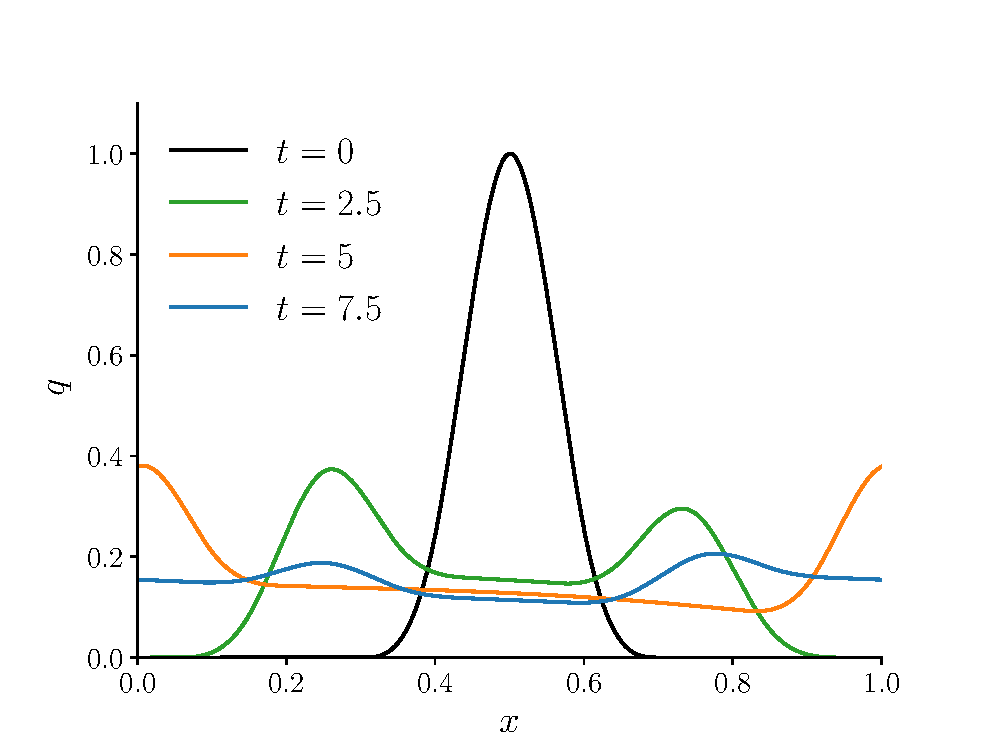
\includegraphics[width=0.5\textwidth]{./figs/wave/solution} & 
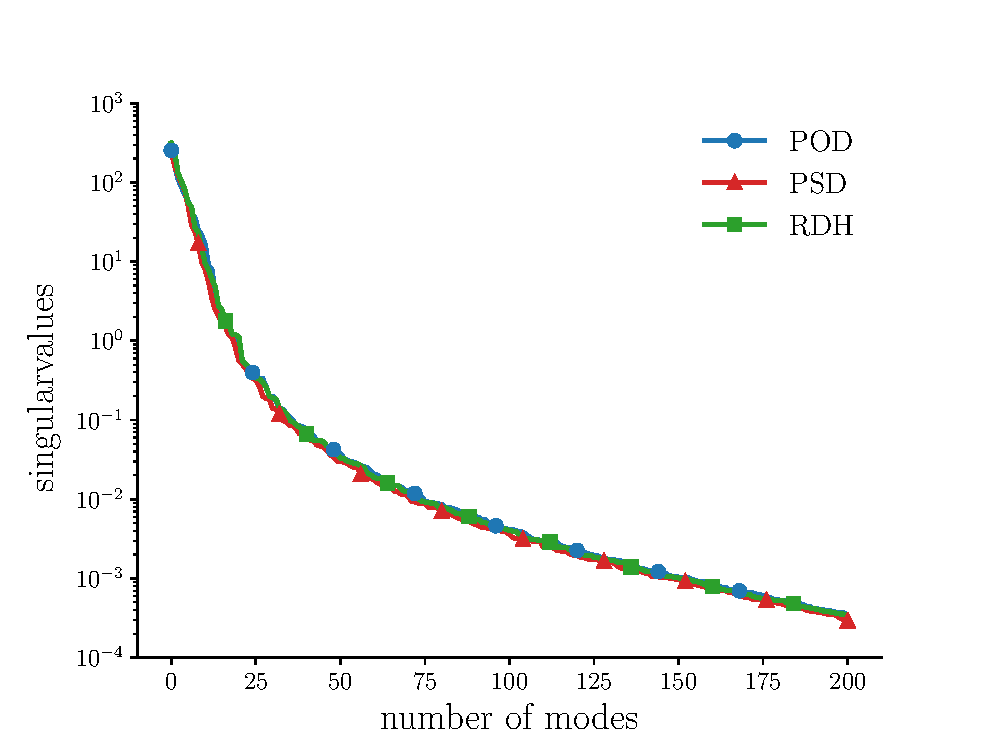
\includegraphics[width=0.5\textwidth]{./figs/wave/singular} \\
(a) & (b) \\
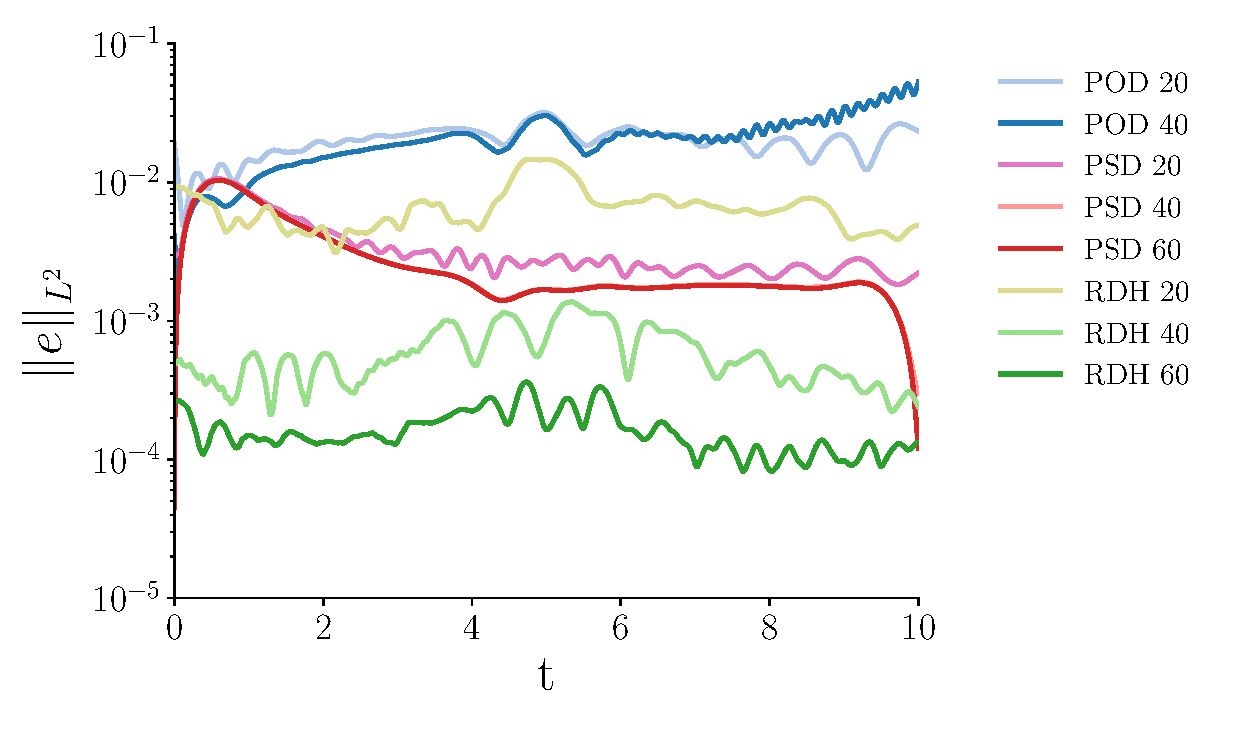
\includegraphics[width=0.5\textwidth]{./figs/wave/error} & 
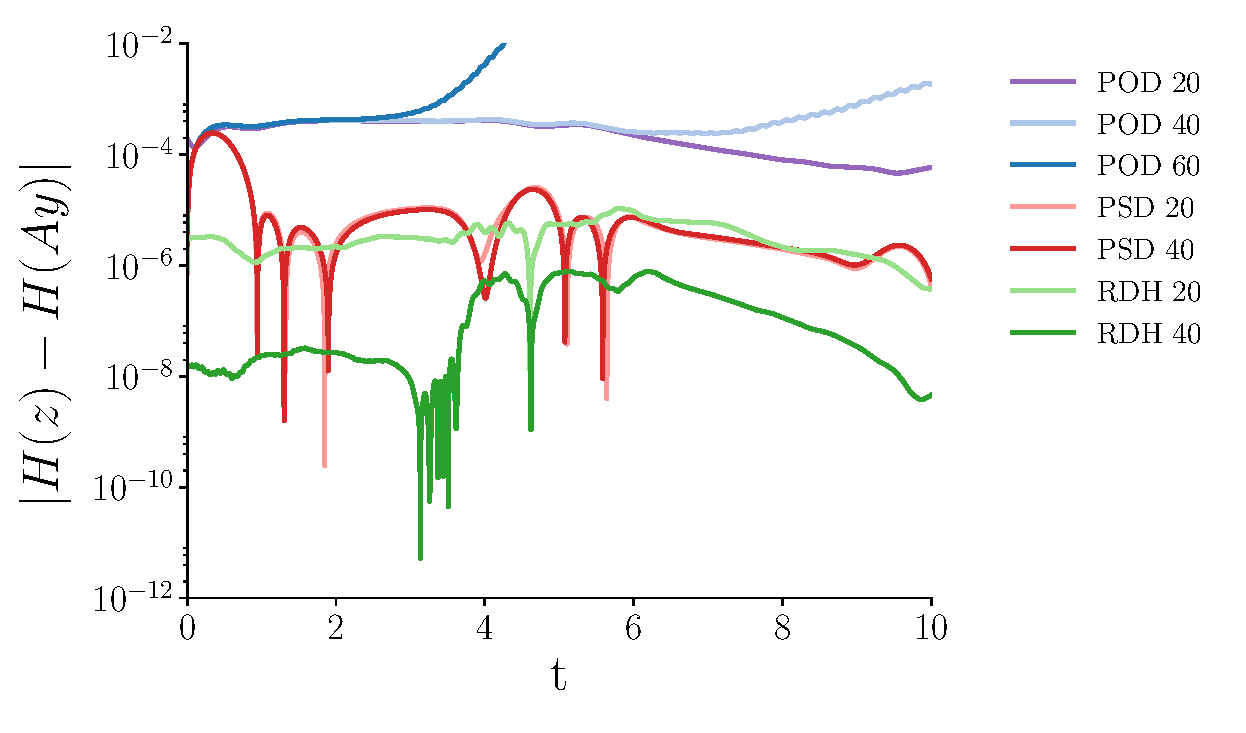
\includegraphics[width=0.5\textwidth]{./figs/wave/energy} \\
(c) & (d) \\
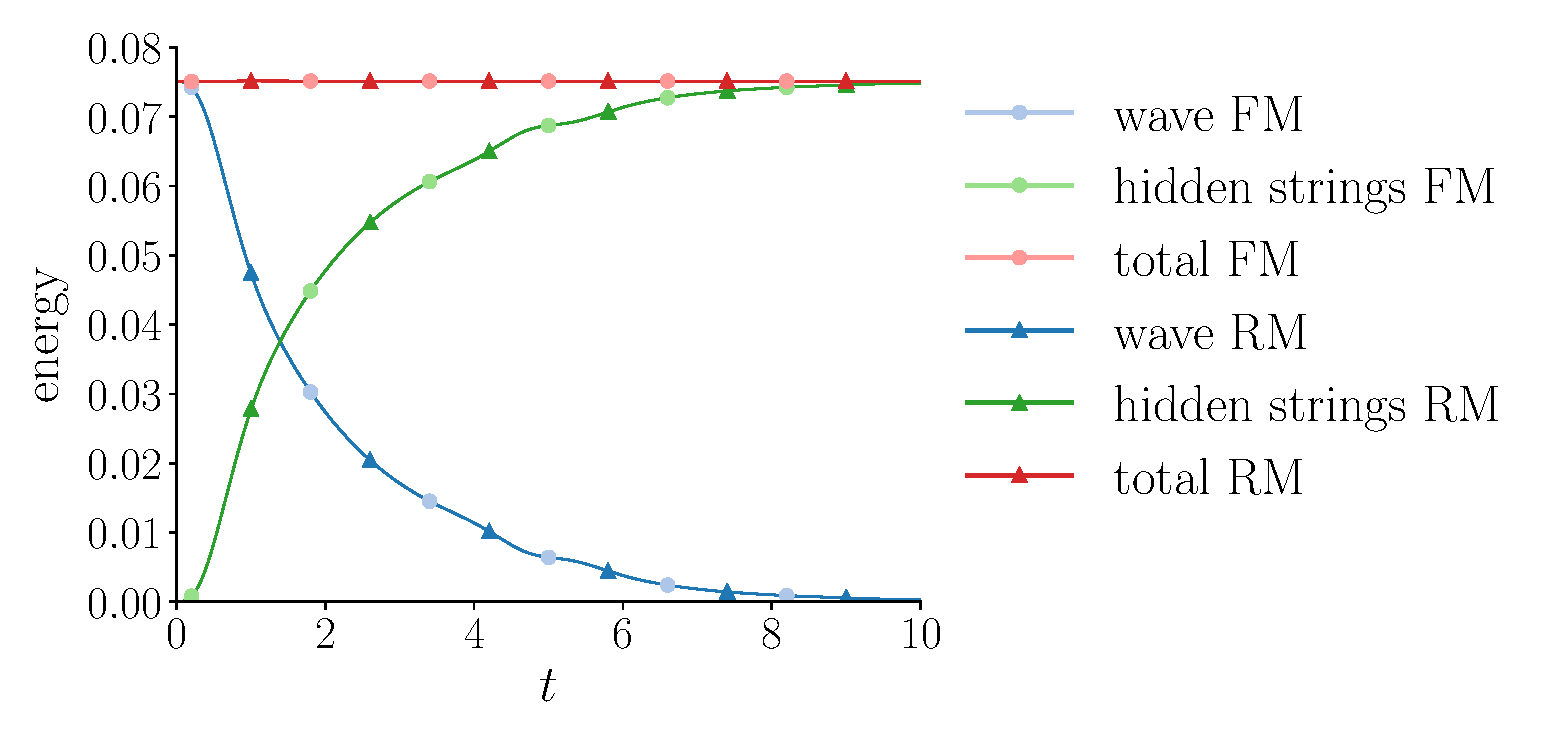
\includegraphics[width=0.55\textwidth]{./figs/wave/energy_conserved} &
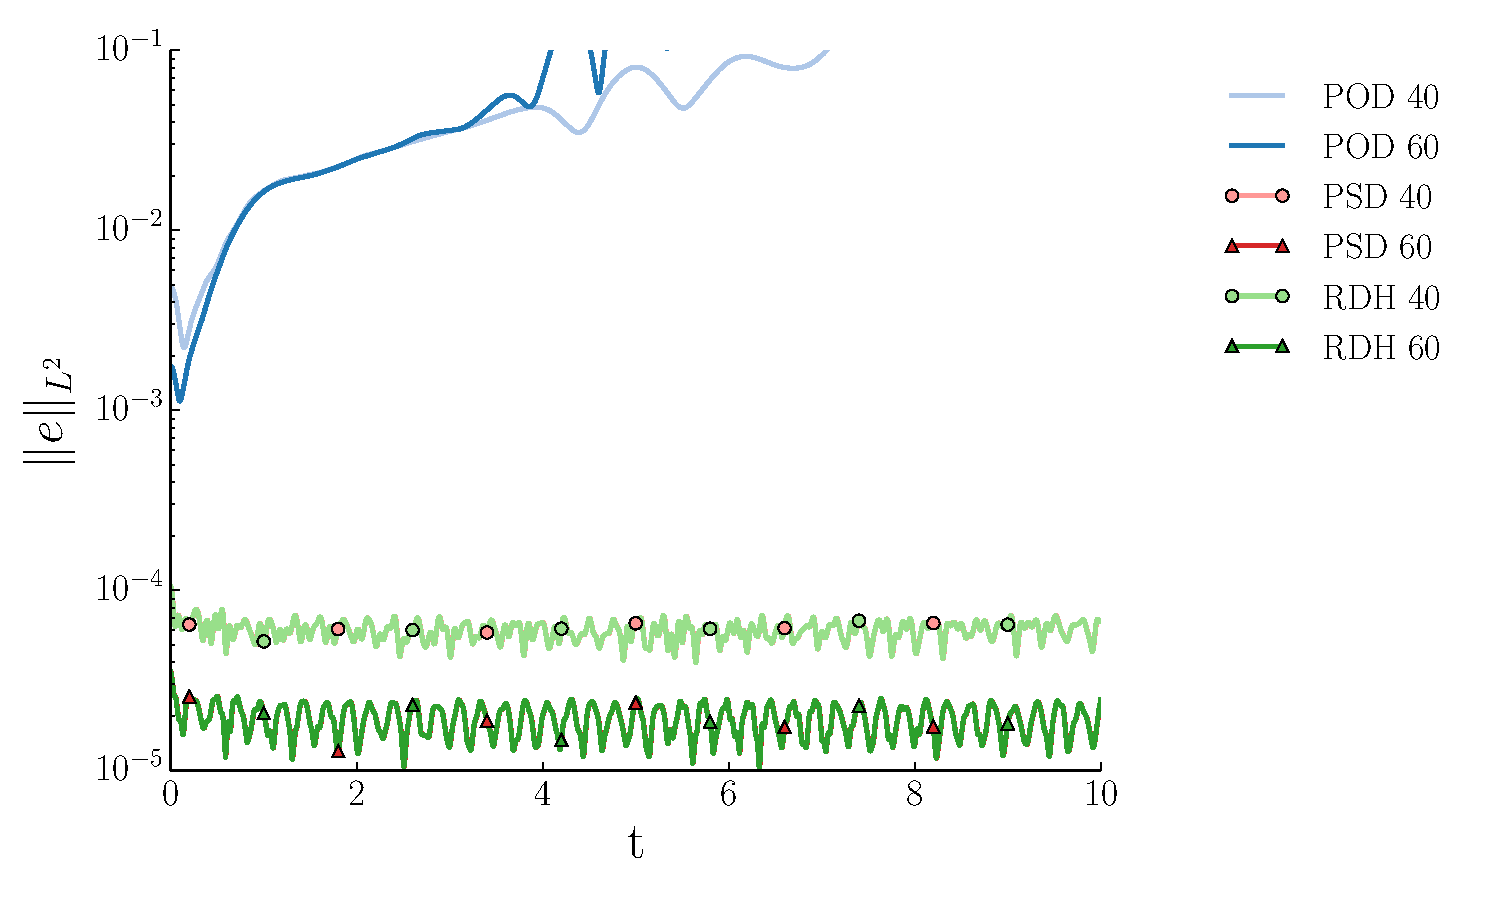
\includegraphics[width=0.45\textwidth]{./figs/wave/error_homo} \\
(e) & (f) 
\end{tabular}
\caption{(a) The solution to the original dissipative wave equation (\ref{eq:4.1}), (b) The decay of the singular values for the POD, the PSD, and the RDH methods, (c) The $L^2$-error for the different methods, (d) Evolution of error in the Hamiltonian for different methods, (e) Energy preservation of the Hamiltonian extension for the original and the reduced system. ``FM'' and ``RM'' refer to the full model and the reduced model, respectively. (f) The $L^2$-error between the solution to the reduced system and the full system in a near-zero dissipation regime.} \label{fig:4.1}
\end{figure}

The second numerical experiment is the dissipative wave equation (\ref{eq:4.1}) in a near-zero dissipation regime. The numerical setting is taken to be identical to the previous numerical experiment, but with the difference that $r_i = 10^{-5}$, for $i=1,\dots,N_{\Delta x}$. Figure \ref{fig:4.1}.(f) shows the $L^2$-error between the solution to the reduced system and the full system, for the POD, the PSD, and the RDH methods. We notice that the POD does not yield a stable reduced system as the symplectic structure is lost via model reduction. Furthermore we notice that error for the PSD and the RDH coincide as the two methods become identical as $\| \chi \|_{\infty}\to 0$.

\subsection{Port-Hamiltonian Systems}
Port-Hamiltonian systems are popular in network modeling and electrical engineering. In the framework of port-Hamiltonian modelling, energy conservation and Hamiltonian structure is the fundamental principle of the dynamics of the system. Ports in the system network then allows the exchange of energy with the environment in the form of sources, capacitors, and dissipations \cite{vanderSchaft:2014:PST:2693645.2693646}. Port-Hamiltonian systems can be viewed as a forced and dissipative Hamiltonian system.
\begin{figure}[t]
\begin{center}
	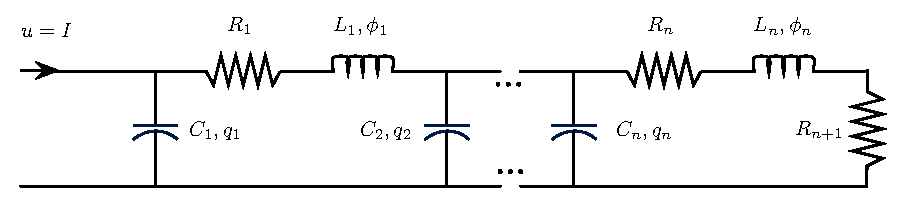
\includegraphics[width=0.7\textwidth]{./figs/porthamil/circuit}
\end{center}
\caption{$n$-dimensional ladder network} \label{fig:4.2}
\end{figure}

Consider the $n$-dimensional linear ladder network in Figure \ref{fig:4.2}. Here $C_i$, $L_i$ and $R_i$, $i=1,\dots,n$, are the capacitance, inductance and resistance of the corresponding capacitors, inductors, and resistors, respectively, and $R_{n+1}$ is the load capacitor. The port-Hamiltonian model of the linear ladder network takes the form
\begin{equation} \label{eq:4.7}
		\dot x = (J_{2n} - R)Q^TQx + u.
\end{equation}
Here $x = (c_1,\phi_1,\dots,c_n,\phi_n)^T$ where $c_i$ and $\phi_i$, for $i=1,\dots,n$, are the charge and the flux of $C_i$ and $L_i$ respectively. $Q$ and $R$ are given as
\begin{equation}
	Q = \text{diag}(C_1^{-1},L_1^{-1},\dots,C_n^{-n},L_n^{-n}), \quad R = \text{diag}(0,R_1,\dots,0,R_n+R_{n+1}),
\end{equation}
$u=(1,0,\dots,0)^T$ is a constant input current and $J_{2n}$ is a skew-symmetric $2n\times 2n$ matrix with -1 and 1 on the superdiagonal and subdiagonal, respectively. 

The energy associated with a port-Hamiltonian system of the form (\ref{eq:4.7}) at time $t$, is given as $H(x(t)) = \frac 1 2 x^T Q^T Q x$. Since $J_{2n}$ is skew symmetric we have that that $\frac d {dt} H(x) = u^T Q^T Q x - x^T Q^T Q R Q^T Q x \leq u^T Q^T Q x$ which is referred to as the \emph{passivity} of the system (\ref{eq:4.7}) \cite{vanderSchaft:1996es,Willems:1972ek}.

Since $J_{2n}$ is full rank, one can always find a coordinate transformation $ x= T \tilde x$ such that $T^{-1} J_{2n} T^{-T} = \mathbb J_{2n}$. The dissipative Hamiltonian formulation of (\ref{eq:4.7}) takes the form
\begin{equation} \label{eq:4.8}
	\dot {\tilde x} = \mathbb J_{2n} \tilde Q^T\tilde Q \tilde x - \tilde Rx + \tilde u,
\end{equation}
where $\tilde Q = QT$, $\tilde R = T^{-1}RT^{-T}Q^TQ$ and $\tilde u = T^{-1} u$. Note that in this case, $\tilde R$ is symmetric and semi-positive definite since $T$ is orthogonal and $R$ is diagonal. The TDD formulation of (\ref{eq:4.8}) takes the form
\begin{equation} \label{eq:4.9}
	\dot{\tilde x} = \mathbb{J}_{2n} \tilde Q^T f(t) + \tilde u, \quad f(t) + \tilde R \int_0^t f(t) = \tilde Q \tilde x.
\end{equation}
The extended Hamiltonian formulation (\ref{eq:2.10.a})-(\ref{eq:2.10.b}) with a quadratic Hamiltonian $H_{\text{ex}}$ can be carried out following Section \ref{sec:2.2}. We note that due to the input $\tilde u$, the Hamiltonian $H_{\text{ex}}$ is time dependent. In fact $\frac{d}{dt} H_{\text{ex}} = \tilde u^T\tilde Q^T \tilde Q \tilde x$. If we define $\overset{\circ}{H}_{\text{ex}} : \mathbb R^{2n}\times \mathcal H^{2n}\times \mathbb R^{2}\to \mathbb R$ as
\begin{equation} \label{eq:4.10}
	\overset{\circ}{H}_{\text{ex}}(\tilde x,\phi,\theta,t,e) = H_{\text{ex}}(\tilde x,\phi,\theta,t) + e, \quad \dot e = - \partial_t H_{\text{ex}},
\end{equation}
it is easily checked that $\frac d {dt} \overset{\circ}{H}_{\text{ex}} =0$ \cite{Hairer:1250576}. However for the time integration of the Hamiltonian system related to $\overset{\circ}{H}_{\text{ex}}$ we can apply a symplectic integrator directly on (\ref{eq:4.10}), since the evolution of $\tilde x$, $\phi$ and $\theta$ does not explicitly depend on $e$. Thus, the passivity of (\ref{eq:4.7}) will be preserved through a symplectic time integration of (\ref{eq:4.9}).

Using an ortho-symplectic reduced basis $A$, the Reduced Dissipative Hamiltonian method can be applied to (\ref{eq:4.9}) to construct a reduced system of the form (\ref{eq:3.12.a})-(\ref{eq:3.12.b}) together with the extended Hamiltonian $\tilde H_{\text{ex}}$. We note that $\frac{d}{dt} \tilde H_{\text{ex}} = (A^+ \tilde u)^T A^T \tilde Q^T \tilde Q A y$, ensuring that the reduced system is passive. Furthermore, the dissipative Hamiltonian structure of the reduced system indicates that the reduced system also carries a port-Hamiltonian structure.

We consider a 100-dimensional ($n=50$) port-Hamiltonian system for the ladder network discussed above. We take $C_i=1$, $L_i = 1$, $R_i=0.2$ for $i=1,\dots,50$, and $R_{51} = 0.4$. We construct the RDH reduced system following Algorithm \ref{alg:3.1}. 

The solution of the RDH method is compared to the main results of \cite{Polyuga:2010gj}, where a passivity-preserving model reduction is developed using a moment matching method at infinity. The charge in $C_1$ is chosen to be the single out put for the moment matching method.

\begin{figure}[t]
\begin{tabular}{cc}
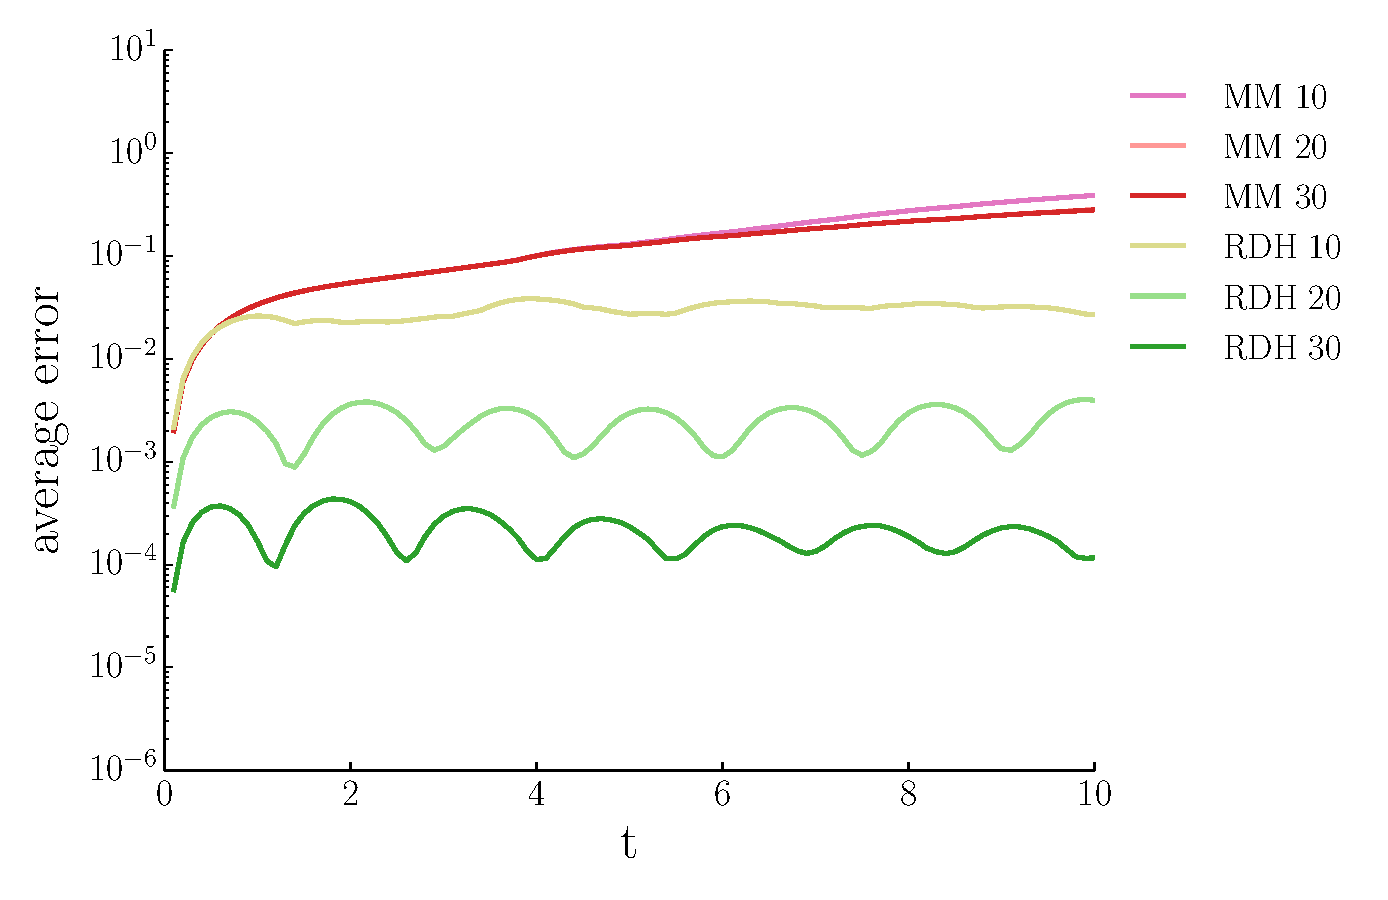
\includegraphics[width=0.5\textwidth]{./figs/porthamil/error_capac} & 
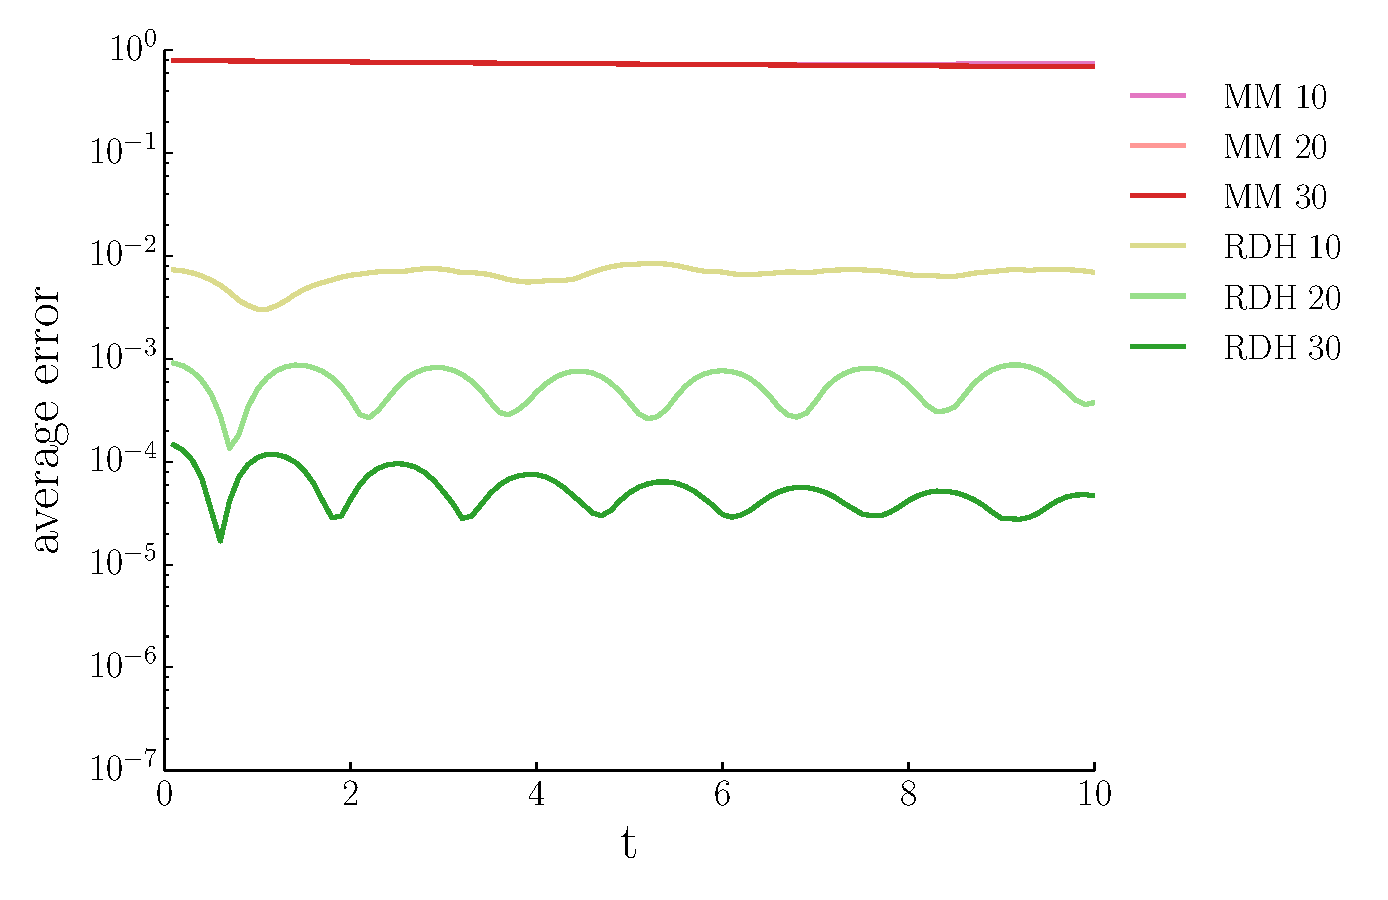
\includegraphics[width=0.5\textwidth]{./figs/porthamil/error_flux} \\
(a) capacitors & (b) inductors \\
\multicolumn{2} {c} {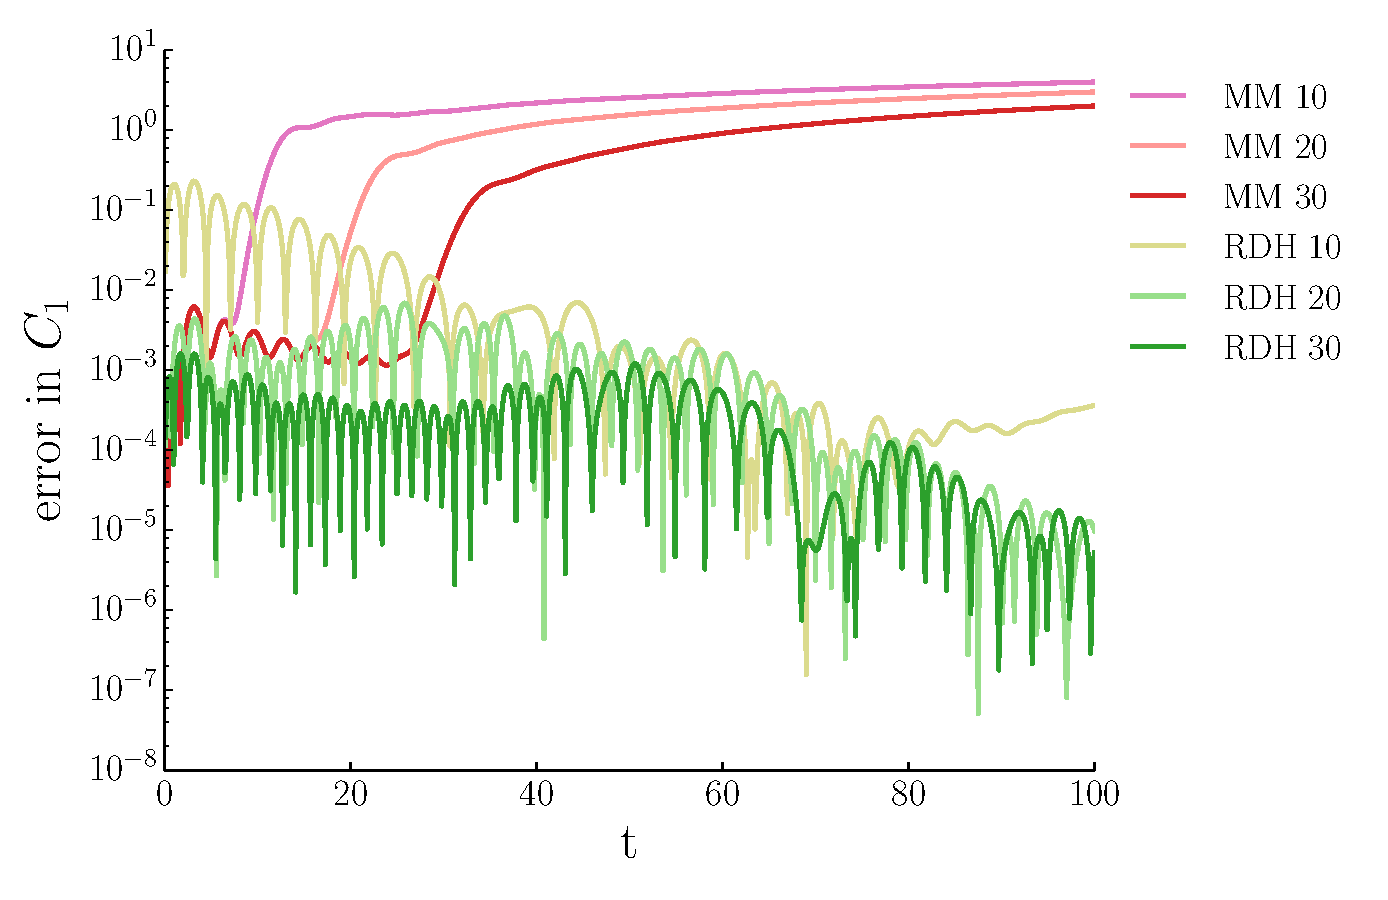
\includegraphics[width=0.5\textwidth]{./figs/porthamil/error1}} \\
\multicolumn{2} {c} {(c) charge in $C_1$} 
\end{tabular}
\caption{Error between the full model and the reduced model obtained by the reduced dissipating Hamiltonian method ``RDH'' and the moment matching method ``MM''. (a) The average error of charge in capacitors in time. (b) the average error of the flux in inductors in time. (c) Error in $C_1$.} \label{fig:4.3}
\end{figure}

Reduced bases of size $2k = 10$, $2k = 20$ and $2k = 30$ are constructed with the RDH and the moment matching method. Figure \ref{fig:4.3}.(c) shows the error in the charge in $C_1$ for the two methods. We observe that although the moment matching method is bounded over long-time integration, the RDH method provides a significantly more accurate solution. In the moment matching method, the passivity of the reduced system implies that the energy of the system will be bounded by the input energy. However, there is no guarantee that the dissipation of energy in the reduced system mimics the one of the original system. On the other hand, the RDH method allows a correct dissipation of energy through the hidden strings and the symplectic time integration in the RDH method guarantees that the total energy is preserved.

Over short-time integration, we notice that the moment matching method with 10 modes provides a more accurate solution than the RDH with 10 modes. Furthermore, the moment matching method with 20 and 30 modes provide a comparable accuracy to the RDH method with 20 and 30 modes. However, the RDH method maintains the high accuracy during long-time integration, while the moment matching method loses up to 3 orders of magnitude in the accuracy, independent of the number of modes.

Figure \ref{fig:4.3}.(a) and Figure \ref{fig:4.3}.(b) show the average temporal error in the charge and flux of the capacitors and inductors, respectively. The RDH method provides a significantly better accuracy compared to the moment matching method. This is because the charge of $C_1$ is specified as the output of interest in the moment matching method and so it is expected that that method provides low accuracy for computing other outputs. On the other hand, the RDH method not only provides high accuracy in computing the charge for $C_1$ but also high accuracy for all components of the system.

